\documentclass[12pt, twoside]{article}
\usepackage[letterpaper, margin=1in, headsep=0.5in]{geometry}
\usepackage[english]{babel}
\usepackage[utf8]{inputenc}
\usepackage{amsmath}
\usepackage{amsfonts}
\usepackage{amssymb}
\usepackage{tikz}
\usetikzlibrary{quotes, angles}
\usepackage{graphicx}
\usepackage{enumitem}
\usepackage{multicol}

\newif\ifmeta
\metatrue %print standards and topics tags

\title{Regents Geometry}
\author{Chris Huson}
\date{September 2020}

\usepackage{fancyhdr}
\pagestyle{fancy}
\fancyhf{}
\renewcommand{\headrulewidth}{0pt} % disable the underline of the header
\raggedbottom


\fancyhead[LE]{\thepage}
\fancyhead[RO]{\thepage \\ Name: \hspace{4cm} \,\\}
\fancyhead[L]{BECA / Dr. Huson / Geometry 06-Analytic-geometry\\* pset ID: 79}

\begin{document}

\subsubsection*{6-12Exam-Analytic-geometry}
\begin{enumerate}
\item Graph and label the two equations. Mark their intersection as an ordered pair.
    \begin{multicols}{2}
      $y =\frac{3}{4}x-5$ \\
      $y=-x+2$
    \end{multicols}     \vspace{0.1cm}
    Write down the slopes of the two lines.
    \begin{multicols}{2}
      $m_1=$ \\
      $m_2=$
    \end{multicols}     \vspace{0.1cm}
    Are the lines parallel, perpendicular, or neither? Justify your answer using the slopes.
    \vspace{3cm}
    \begin{center}
      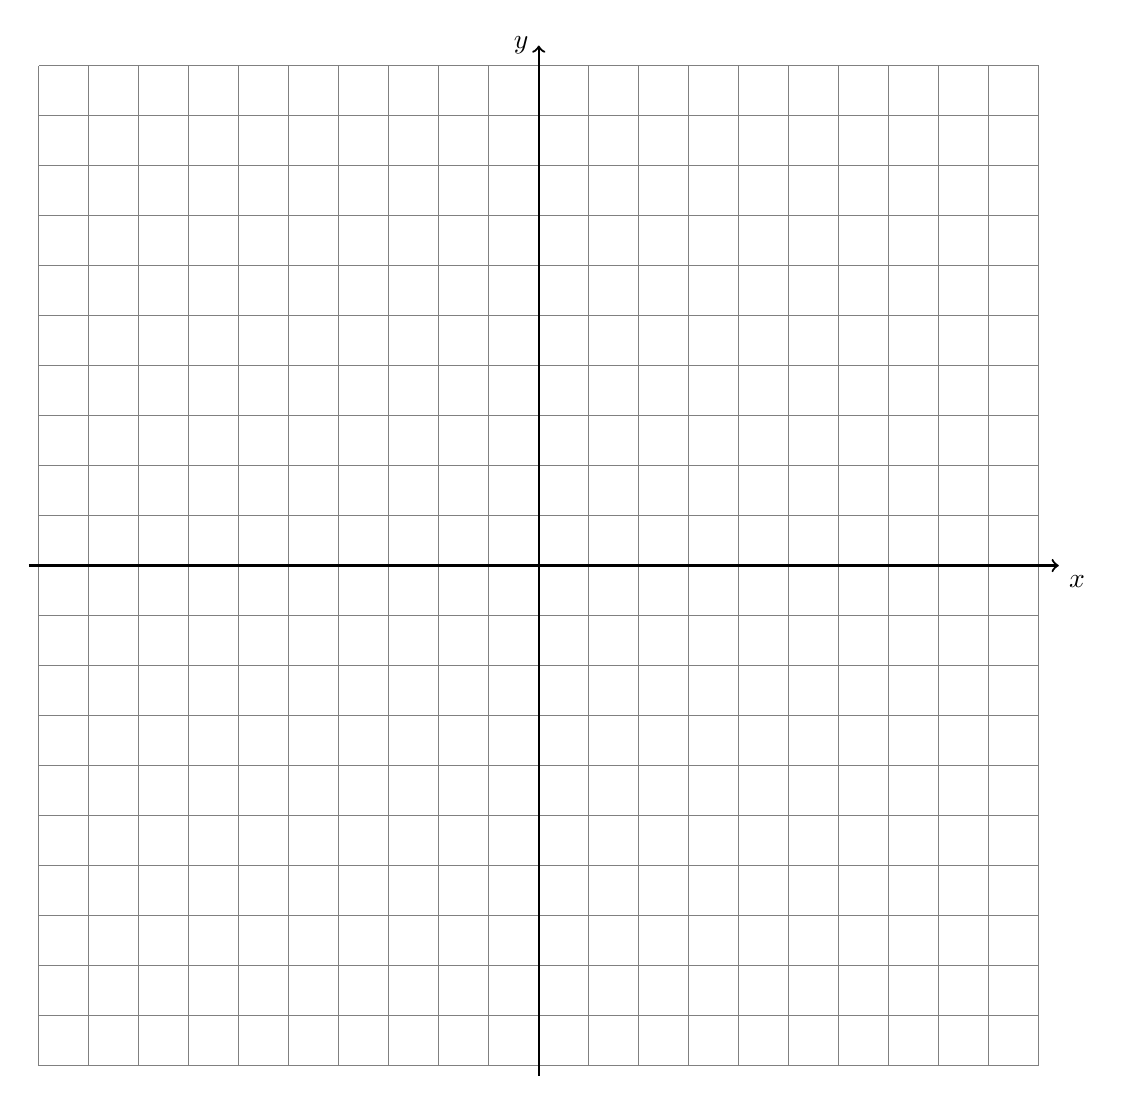
\begin{tikzpicture}[scale=.635]
        \draw [help lines] (-10,-10) grid (10,10);
        \draw [thick, ->] (-10.2,0) -- (10.4,0) node [below right] {$x$};
        \draw [thick, ->] (0,-10.2)--(0,10.4) node [left] {$y$};
      \end{tikzpicture}
    \end{center}

\newpage
\item Graph and label the two equations. Mark their intersection as an ordered pair.
      \begin{multicols}{2}
        $y =-\frac{1}{3}x+4$ \\[0.25cm]
        $3x-y=6$ \\
        Are the lines parallel, perpendicular, or neither? Justify your answer using the slopes.
      \end{multicols}     \vspace{0.1cm}
      \vspace{1cm}
      \begin{flushright} %4 quadrant regents grid w T-Chart
      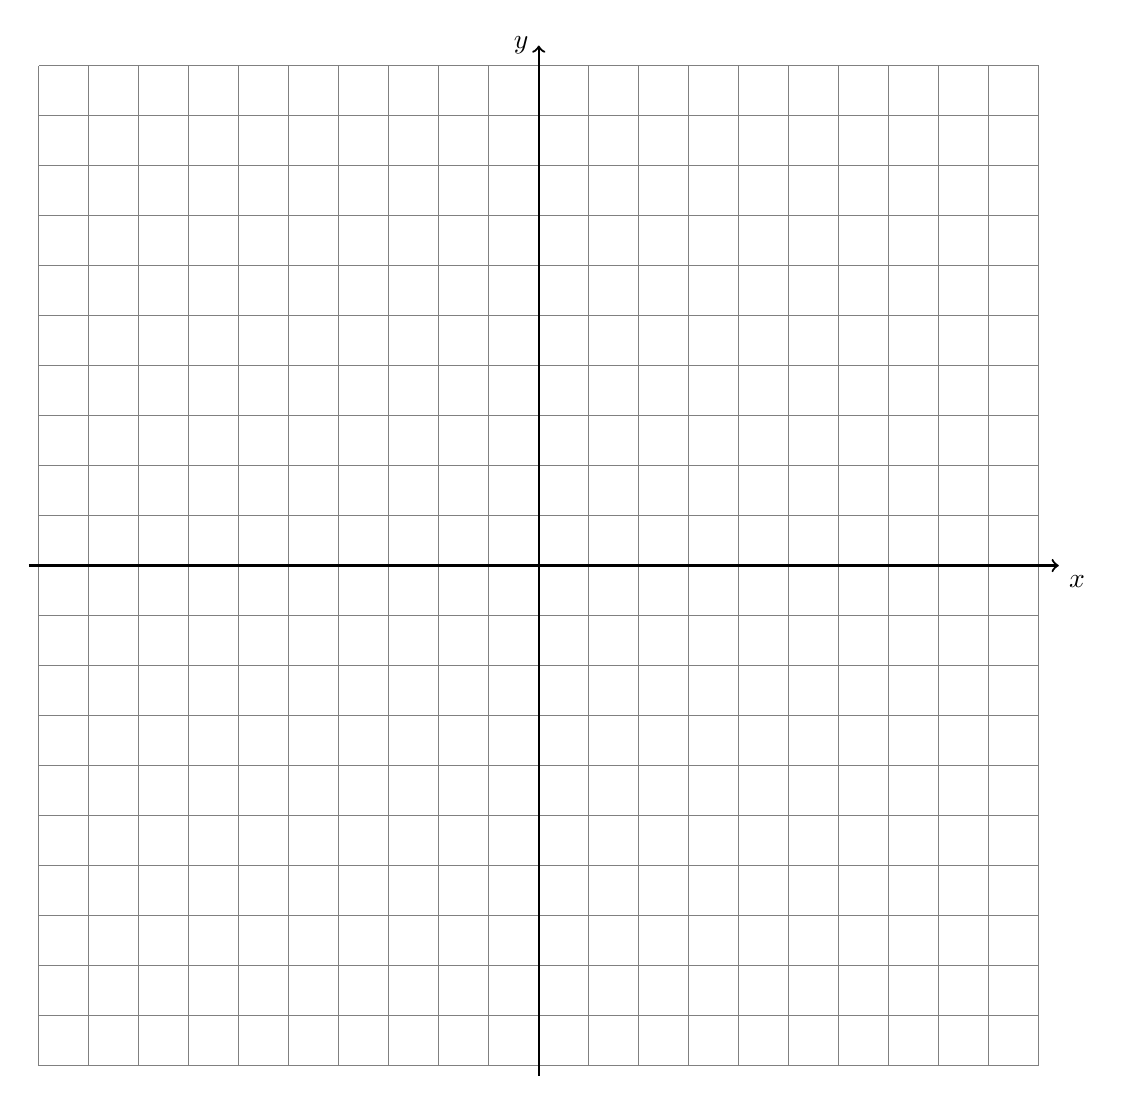
\begin{tikzpicture}[scale=.635]
        \draw [help lines] (-10,-10) grid (10,10);
        \draw [thick, ->] (-10.2,0) -- (10.4,0) node [below right] {$x$};
        \draw [thick, ->] (0,-10.2)--(0,10.4) node [left] {$y$};
      \end{tikzpicture}
      \end{flushright}

\item The line $l$ has the equation $y=-\frac{3}{5}x+3$.
  \begin{enumerate}
    \item What is the slope of the line $k$, given $k \parallel l$?
    \vspace{0.5cm}
    \item What is the slope of the line $j$, given $j \perp l$?
    \vspace{0.5cm}
  \end{enumerate}

\newpage
\item Apply a dilation mapping $\triangle ABC \rightarrow \triangle A'B'C'$ with a factor of $k=3$ centered at the origin. Draw and label the image on the grid and make a table of the coordinates.
    \begin{flushright} %4 quadrant regents grid w T-Chart
    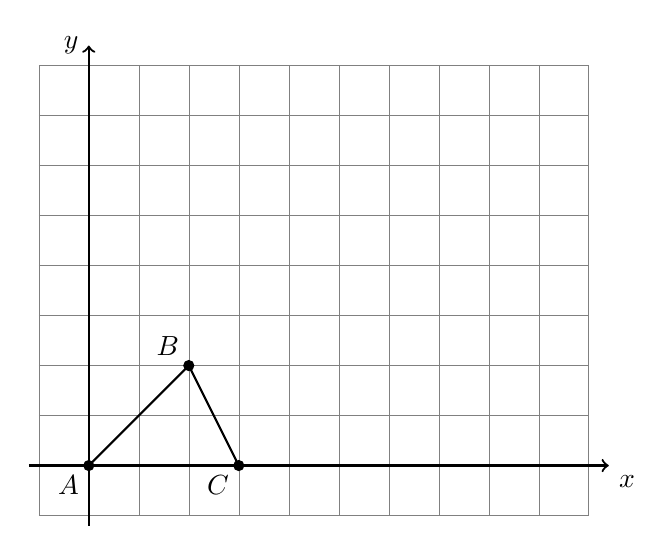
\begin{tikzpicture}[scale=.635]
      \draw [help lines] (-1,-1) grid (10,8);
      \draw [thick, ->] (-1.2,0) -- (10.4,0) node [below right] {$x$};
      \draw [thick, ->] (0,-1.2)--(0,8.4) node [left] {$y$};
      \draw [thick] (0,0)--(3,0)--(2,2)--cycle;
      \draw [fill] (0,0) circle [radius=0.1]node[below left]{$A$};
      \draw [fill] (3,0) circle [radius=0.1]node[below left]{$C$};
      \draw [fill] (2,2) circle [radius=0.1]node[above left]{$B$};
    \end{tikzpicture}
    \end{flushright} \vspace{1cm}
    
\item Find the image of $P(-2,7)$ after the translation $(x,y) \rightarrow (x+5,y-2)$.  \vspace{3cm}

\item What transformation maps $\triangle ABC$ onto $\triangle DEF$, shown below? Fully specify the transformation. \\[0.25cm]
  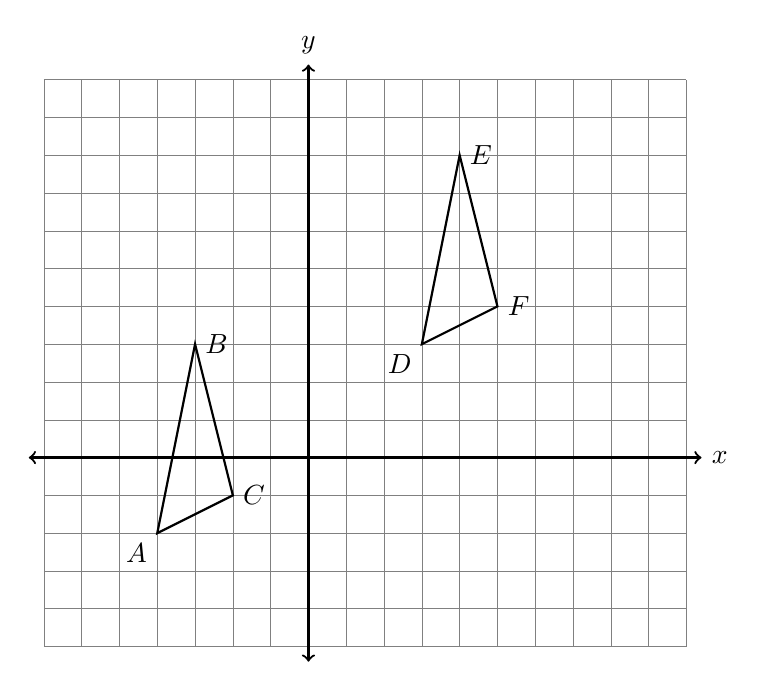
\begin{tikzpicture}[scale=.48]
    \draw [help lines] (-7,-5) grid (10,10);
    \draw [thick, <->] (-7.4,0) -- (10.4,0) node [right] {$x$};
    \draw [thick, <->] (0,-5.4)--(0,10.4) node [above] {$y$};  
    \draw [thick]
    (-4,-2) node[below left] {$A$}--
    (-3,3) node[right] {$B$}--
    (-2,-1) node[right] {$C$}--cycle;  
    \draw [thick]
    (3,3) node[below left] {$D$}--
    (4,8) node[right] {$E$}--
    (5,4) node[right] {$F$}--cycle; 
  \end{tikzpicture}

\newpage
\item Translate $\triangle ABC$ to the right six units and down two units. Make a table of the coordinates and plot and label the image on the axes.
  \begin{flushright}
    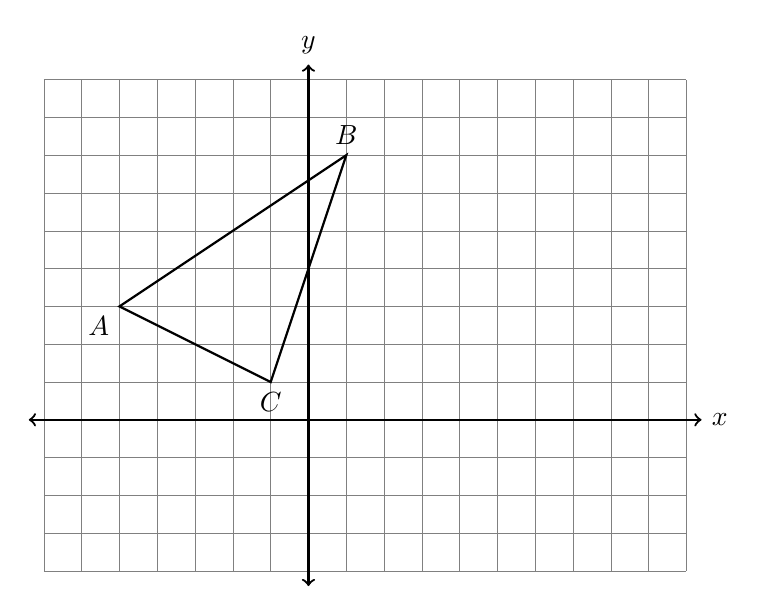
\begin{tikzpicture}[scale=.48]
      \draw [help lines] (-7,-4) grid (10,9);
      \draw [thick, <->] (-7.4,0) -- (10.4,0) node [right] {$x$};
      \draw [thick, <->] (0,-4.4)--(0,9.4) node [above] {$y$};  
      \draw [thick]
        (-5,3) node[below left] {$A$}--
        (1,7) node[above] {$B$}--
        (-1,1) node[below] {$C$}--cycle;  
  \end{tikzpicture}
  \end{flushright}

\item A translation maps $P(-5, 3) \rightarrow P'(6,1)$. What is the image of $Q(1,9)$ under the same translation? \vspace{1cm}

\item A dilation maps triangle $KLM$ onto triangle $PQR$, with $KM=5$, $LM=4$, $PR=10$. \vspace{0.5cm}
    \begin{multicols}{2}
      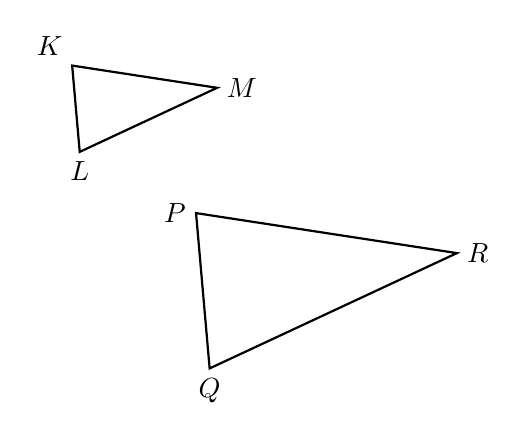
\begin{tikzpicture}[scale=0.55]
        \coordinate [label=above left:$K$](A) at (95:2);
        \coordinate [label=below:$L$](B) at (0, 0);
        \coordinate [label=right:$M$](C) at (25:3.5);
        \draw [thick] (A)--(B)--(C)--cycle;
        \draw [thick, xshift=3cm, yshift=-5cm, scale=1.8] (95:2) node[left]{$P$}--
        (0,0) node[below]{$Q$}--
        (25:3.5) node[right]{$R$}--cycle;
      \end{tikzpicture}\\
      Complete each mapping or equivalence.
      \begin{enumerate}
        \item $L \rightarrow$ \rule{2cm}{0.15mm} \vspace{0.25cm}
        \item $\angle K \cong$ \rule{2cm}{0.15mm} \vspace{0.75cm}
        \item $QR=$ \rule{2cm}{0.15mm}
        %\item Justify $\triangle KLM \sim \triangle PQR$. Use the words ``maintains angles" and ``dilation''. \qquad \qquad (2 stars)
      \end{enumerate}
    \end{multicols} %\vspace{2cm}
  
\item Given $\triangle ABC \sim \triangle DEF$. $m\angle A = 33^\circ$ and $m\angle B = 66^\circ$. Find the measure of $\angle D$.
    
\newpage
\item A dilation centered at $A$ maps $\triangle ABC \rightarrow \triangle ADE$. Given the sides of the preimage, $AC = 6$, $BC = 4$, $AB = 8$, and of $DE = 10$ find the scale factor $k$ and the lengths $AD$ and $AE$. Then find $CE$ and $BD$. 
  \begin{multicols}{2}
    \begin{enumerate}
      \item $k=$ \vspace{0.3cm}
      \item $AD=$ \vspace{0.3cm}
      \item $AE=$ \vspace{0.3cm}
      \item $CE=$
      \item $BD=$
    \end{enumerate}
  \begin{flushright}
    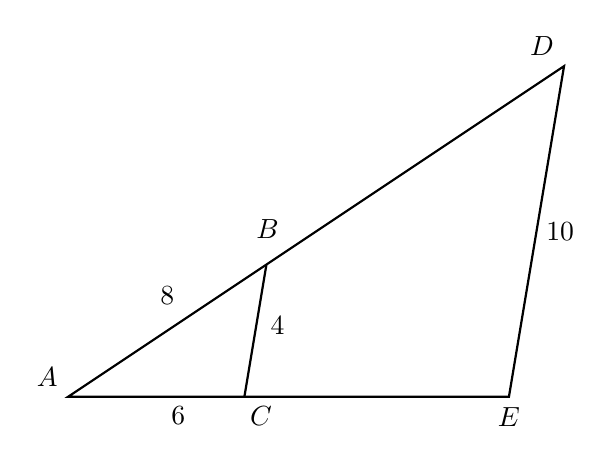
\begin{tikzpicture}[scale=0.7]
      \draw [-, thick] (0,0) node[above left]{$A$}--
      (8,0) node[below]{$E$}--
      (9,6) node[above left]{$D$}--cycle;
      \draw [thick] (3.2,0)--(3.6,2.4);
      \node at (3.5,0) [below]{$C$};
      \node at (4,2.7) [above left]{$B$};
      \node at (2, 0) [below]{$6$};
      \node at (1.8,1.5) [above]{$8$};
      \node at (8.5, 3) [right]{$10$};
      \node at (3.5, 1.3) [right]{$4$}; \vspace{1cm}
    \end{tikzpicture}
  \end{flushright} 
\end{multicols}\vspace{1.5cm}
  
\item Triangle $ABC$ is dilated with a scale factor of $k$ centered at $A$, yielding $\triangle ADE$, as shown. Given $AB=12$, $BC=16$, $AC=20$, and $BD=3$. \\[0.25cm] Find the scale factor $k$ and the segment lengths $DE$ and $CE$.
  \begin{flushright} \emph{(the diagram is not to scale)} \end{flushright}
    \begin{flushright}
      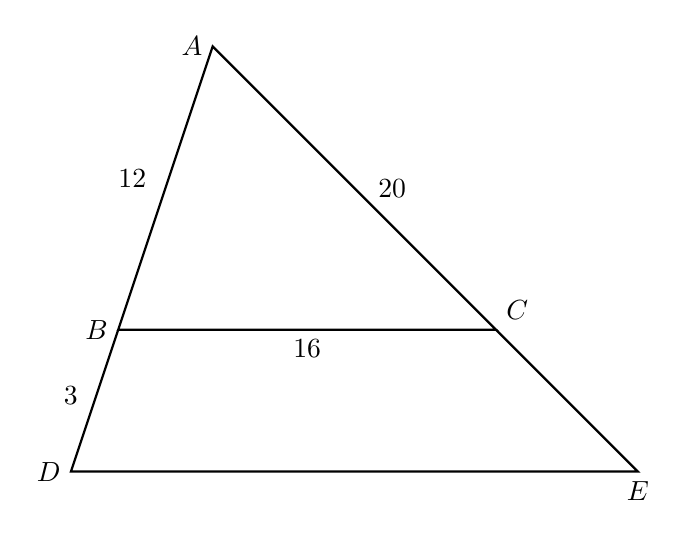
\begin{tikzpicture}[scale=0.6]
        \draw [thick]
        (0,0)node[left]{$B$}--
        (8,0)node[above right]{$C$}--
        (2,6)node[left]{$A$}--cycle;
        \draw [thick]
        (0,0)--
        (-1,-3)node[left]{$D$}--
        (11,-3)node[below]{$E$}--(8,0);
        \node at (4,0)[below]{$16$};
        \node at (5.3, 3)[right]{$20$};
        \node at (0.3, 2.8)[above]{$12$};
        \node at (-1,-1)[below]{$3$};
      \end{tikzpicture}
    \end{flushright} \vspace{2.5cm}

  \newpage
\item As shown, $\overline{AB}$ has endpoints with coordinates $A(2,1)$ and $B(8, 7)$. Show the calculation for the coordinates of the midpoint $M$ of $\overline{AB}$. Mark and label it on the graph.
      \begin{flushright}
        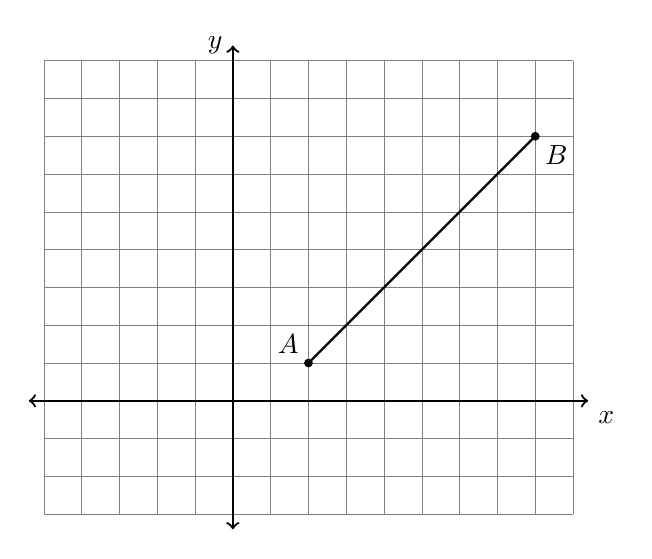
\begin{tikzpicture}[scale=.48]
          \draw [help lines] (-5,-3) grid (9,9);
          \draw [thick, <->] (-5.4,0) -- (9.4,0) node [below right] {$x$};
          \draw [thick, <->] (0,-3.4)--(0,9.4) node [left] {$y$};
          \draw [thick] (2,1)--(8,7);
          \draw [fill] (2,1) circle [radius=0.1] node[above left] {$A$};
          \draw [fill] (8,7) circle [radius=0.1] node[below right] {$B$};
        \end{tikzpicture}
      \end{flushright}

\item $A(-2,5)$ is one endpoint of $\overline{AB}$. The segment's midpoint is $M(3,3)$, as shown below.  
  \begin{multicols}{2}
    \begin{enumerate}
    \item What translation maps \\[0.25cm] $A(-2,5) \rightarrow M(3,3)$?
    \item Find the other endpoint, $B$. \vspace{2cm}
    \end{enumerate}
    \begin{flushright}
      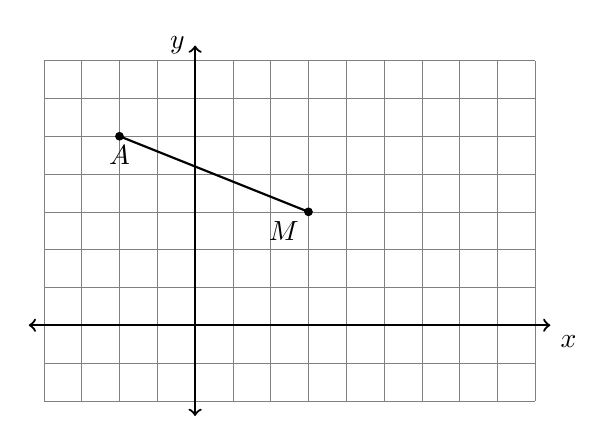
\begin{tikzpicture}[scale=.48]
        \draw [help lines] (-4,-2) grid (9,7);
        \draw [thick, <->] (-4.4,0) -- (9.4,0) node [below right] {$x$};
        \draw [thick, <->] (0,-2.4)--(0,7.4) node [left] {$y$};
        \draw [thick] (-2,5)--(3,3);
        \draw [fill] (-2,5) circle [radius=0.1] node[below] {$A$};
        \draw [fill] (3,3) circle [radius=0.1] node[below left] {$M$};
      \end{tikzpicture}
    \end{flushright}
  \end{multicols}

\item In the diagram below, $\overline{AD}$ has endpoints with coordinates $A(-3,0)$ and $D(6,3)$. What points $B$ and $C$ trisect $\overline{AD}$ into three congruent segments? Mark and label them on the graph. State their coordinates.
    \begin{flushright}
      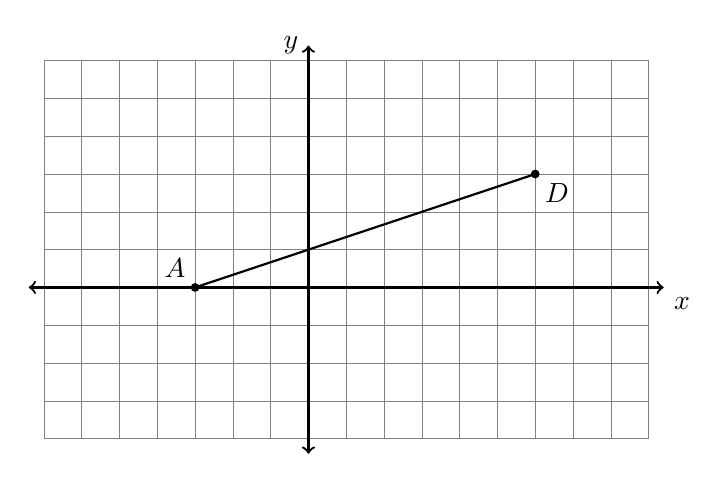
\begin{tikzpicture}[scale=.48]
        \draw [help lines] (-7,-4) grid (9,6);
        \draw [thick, <->] (-7.4,0) -- (9.4,0) node [below right] {$x$};
        \draw [thick, <->] (0,-4.4)--(0,6.4) node [left] {$y$};
        \draw [thick] (-3,0)--(6,3);
        \draw [fill] (-3,0) circle [radius=0.1] node[above left] {$A$};
        \draw [fill] (6,3) circle [radius=0.1] node[below right] {$D$};
      \end{tikzpicture}
    \end{flushright}

\newpage
\item Given $\triangle ABC$, find the lengths of its sides. $A(1,2)$, $B(9,8)$, $C(9,2)$.
  \begin{enumerate}
    \begin{multicols}{2}
    \item   $AC=$ \vspace{0.6cm}
    \item   $BC=$ \vspace{0.75cm}
    \item   Use the formula for distance: \\$\displaystyle d=\sqrt{(x_2-x_1)^2+(y_2-y_1)^2}$ \\$AB=$ \vspace{2.5cm}
      \begin{center}
        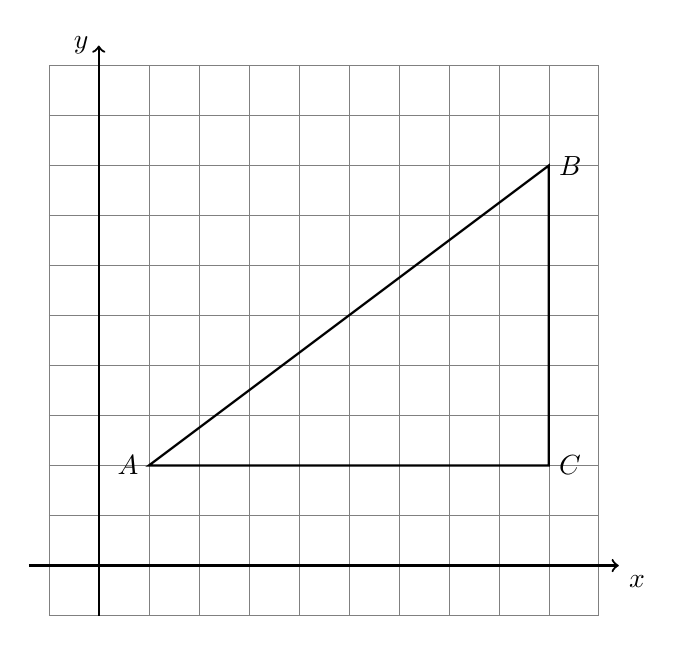
\begin{tikzpicture}[scale=.635]
          \draw [help lines] (-1,-1) grid (10,10);
          \draw [thick, ->] (-1.4,0) -- (10.4,0) node [below right] {$x$};
          \draw [thick, ->] (0,-1)--(0,10.4) node [left] {$y$};
          \draw [thick] (1,2)node[left]{$A$}--
          (9,8)node[right]{$B$}--
          (9,2)node[right]{$C$}--
          cycle;
        \end{tikzpicture}
        \end{center}
    \end{multicols}
  \end{enumerate}
  \vspace{1cm} 

\item Given two parallel lines and a transversal, as shown below. Given $m\angle 1 = 117$.
  \begin{center}
  \begin{tikzpicture}
    \draw [<->, thick] (1,2)--(9,2);
    \draw [<->, thick] (0,0)--(8,0);
    \draw [<->, thick] (4,-1)--(5.5,3);
    \node at (4.5,0.3) [left]{$5$};
    \node at (4.5,0.3) [right]{$6$};
    \node at (4.3,-0.3) [left]{$7$};
    \node at (4.3,-0.3) [right]{$8$};
    \node at (5.2,2) [above left]{$1$};
    \node at (5.2,2) [above right]{$2$};
    \node at (5,2) [below left]{$3$};
    \node at (5,2) [below right]{$4$};
  \end{tikzpicture}
  \end{center}
  \begin{enumerate}
    \item Find the measure $m\angle 2$. \vspace{0.5cm}
    \item Find the measure $m\angle 4$. \vspace{0.5cm}
    \item Find the measure $m\angle 5$.  \vspace{0.5cm}
    \item Given $m\angle 8 = (5x-8)^\circ$. Find $x$. \vspace{3.5cm}
  \end{enumerate}

  \newpage
\item Given isosceles $\triangle ABC$ with $\overline{AB} \cong \overline{BC}$, $m\angle A = x$, $m\angle B = 63$, and $m\angle C=y$. Mark and label the diagram, and then find $x$ and $y$. \hfill (\emph{the diagram is not to scale})
  \begin{flushright}
  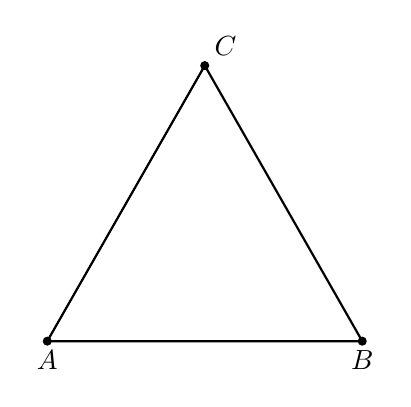
\begin{tikzpicture}[scale=1]
    \draw [thick](0,0)--(4,0)--(2,3.5)--(0,0);
    \draw [fill] (0,0) circle [radius=0.05] node[below]{$A$};
    \draw [fill] (4,0) circle [radius=0.05] node[below]{$B$};
    \draw [fill] (2,3.5) circle [radius=0.05] node[above right]{$C$};
  \end{tikzpicture}
  \end{flushright}

\item Given isosceles $\triangle RSU$ with $\overline{RS} \cong \overline{US}$. If $m\angle UST=140$ find $m\angle R$. (mark and label the diagram) \hfill (\emph{the diagram is not to scale})
  \begin{flushright}
  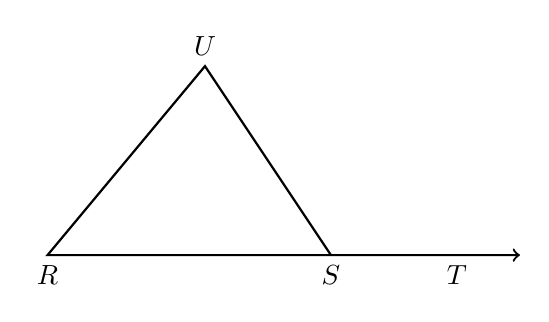
\begin{tikzpicture}[scale=0.8]
    %\draw [->, thick] (0,0)--(5,5);
    \draw [<-, thick] (8,0)--
      (7,0) node[below]{$T$}--
      (0.5,0) node[below]{$R$}--
      (3,3) node[above]{$U$}--
      (5,0) node[below]{$S$};
  \end{tikzpicture}
  \end{flushright} \vspace{1cm}

\item Given parallel lines $\overleftrightarrow{AB} \parallel \overleftrightarrow{CDE}$ with $\overline{AC} \cong \overline{CD}$. If $m\angle BAD=55$ find $m\angle ACD$. (completely mark and label the diagram)
    \begin{flushright}
    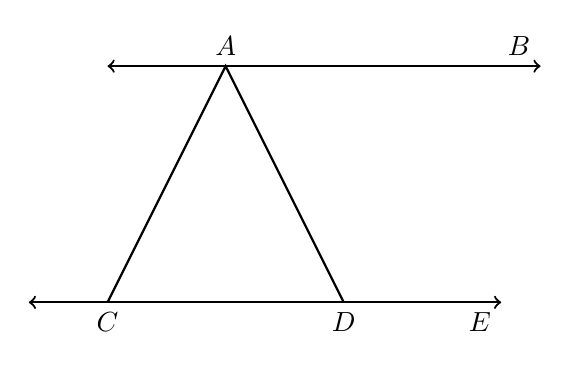
\begin{tikzpicture}
      \draw [<->, thick] (1,3)--(6.5,3) node[above left]{$B$};
      \draw [<->, thick] (0,0)--
        (5,0)--
        (6,0) node[below left]{$E$};
      \draw [-, thick] (1,0) node[below]{$C$}--
        (2.5,3) node[above]{$A$}--
        (4,0) node[below]{$D$};
    \end{tikzpicture}
    \end{flushright} \vspace{1.5cm}
    
\newpage
%\subsubsection*{Early Finishers}
\item Two parallel lines intersect a second set of parallel lines. Given $m\angle 1 = x$ and $m\angle 2 = 2x-24$, find the measure of $\angle 4$. 
    \begin{flushright}
      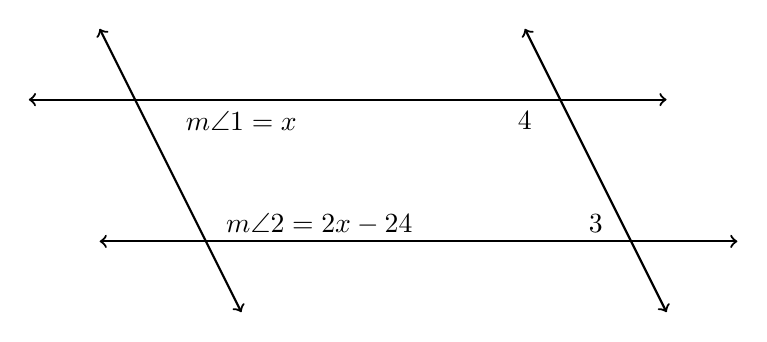
\begin{tikzpicture}[scale=0.9]
        \draw [<->, thick] (3,0)--(12,0);
        \draw [<->, thick] (2,2)--(11,2);
        \draw [<->, thick] (5,-1)--(3,3);
        \draw [<->, thick] (11,-1)--(9,3);
        \node at (5, 1.7){$m\angle 1 = x$};
        \node at (6.1, 0.25){$m\angle 2 = 2x-24$};
        \node at (10, 0.25){$3$};
        \node at (9, 1.7){$4$};
      \end{tikzpicture}
    \end{flushright} \vspace{2cm}

\item Reflect $\triangle ABC$ over the $x$-axis, then translate it by $(x,y) \rightarrow (x+9, y+3)$. Make a table of the coordinates showing $\triangle ABC \rightarrow \triangle A'B'C' \rightarrow \triangle A''B''C''$ and plot and label the image on the axes.
  \begin{flushright}
      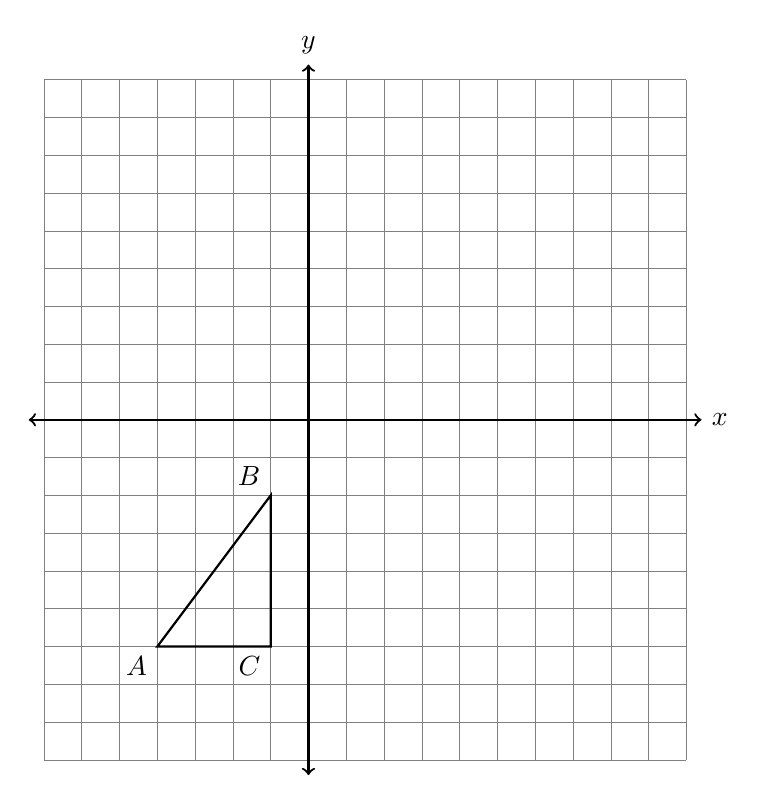
\begin{tikzpicture}[scale=.48]
      \draw [help lines] (-7,-9) grid (10,9);
      \draw [thick, <->] (-7.4,0) -- (10.4,0) node [right] {$x$};
      \draw [thick, <->] (0,-9.4)--(0,9.4) node [above] {$y$};  
      \draw [thick]
        (-4,-6) node[below left] {$A$}--
        (-1,-2) node[above left] {$B$}--
        (-1,-6) node[below left] {$C$}--cycle;  
    \end{tikzpicture}
  \end{flushright}

\newpage
\item In the diagram below, $\triangle ABC$ with sides of 10, 13, and 16, is mapped onto $\triangle DEF$ after a clockwise rotation of $90^\circ$ about point $P$. \\*[0.25cm]
  If $DE=3x+1$, what is the value of $x$? 
      \begin{flushright}
        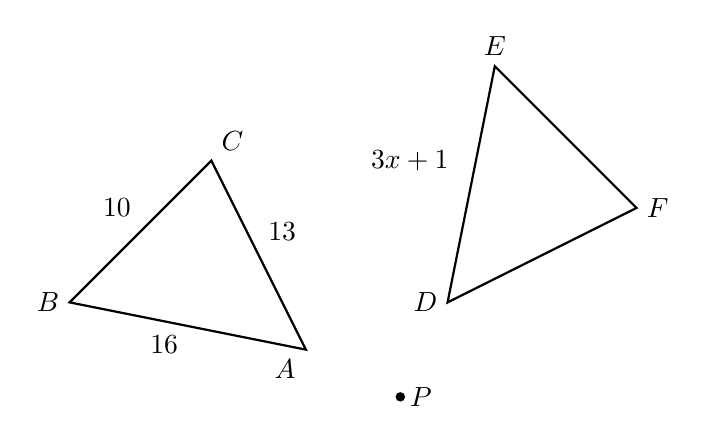
\begin{tikzpicture}[scale=.6]
          %\draw [thick, <->] (-7.4,0) -- (10.4,0) node [right] {$x$};
          %draw [thick, <->] (0,-5.4)--(0,10.4) node [above] {$y$};
          \fill (0,0) circle[radius=0.1] node[right]{$P$};
          \draw [thick]
            (-2,1) node[below left] {$A$}--
            (-7,2) node[left] {$B$}--
            (-4,5) node[above right] {$C$}--cycle;
            \node at (-5,1.5)[below]{16};
            \node at (-6,4){10};
            \node at (-2.5,3.5){13};
            \node at (0.2,5){$3x+1$};
          \draw [thick]
            (1,2) node[left] {$D$}--
            (2,7) node[above] {$E$}--
            (5,4) node[right] {$F$}--cycle;
        \end{tikzpicture}
      \end{flushright}  \vspace{1cm}

\item Given $\triangle ABP \sim \triangle JKP$ as shown below. $AB=9.6$, $AP=12.0$, $BP=6.3$, and $JP=27.0$. Find $JK$.
  \begin{flushright}
  \begin{tikzpicture}[scale=1.4]
      \draw [thick]
        (-0.25,-1)node[below left]{$B$}--
        (0.5,2)node[left]{$K$}--
        (4,0)node[below left]{$J$}--
        (0,0)node[above left]{$P$}--
        (-2,0)node[left]{$A$}--cycle;
    \end{tikzpicture}
    \end{flushright}
    \vspace{2cm}

\newpage
  \subsubsection*{Spicy Regents problems: Using slope to prove a parallelogram}
\item In this problem use the following theorem (copy it at the bottom of the page after your calculations): \\*[0.25cm]
    \emph{A quadrilateral is a parallelogram if and only if it's opposite sides are parallel.}\\*[0.5cm]
    Shown below is quadrilateral $ABCD$, $A(2,-1)$, $B(5,1)$, $C(1,6)$, and $D(-2,4)$. \\*[0.25cm]
    Prove it is a parallelogram by
    \begin{enumerate}
      \item finding the slope of each of the four sides,
      \item stating which sides are parallel,
      \item copying the theorem as your conclusion.
    \end{enumerate}
    \begin{flushright} %4 quadrant regents grid
      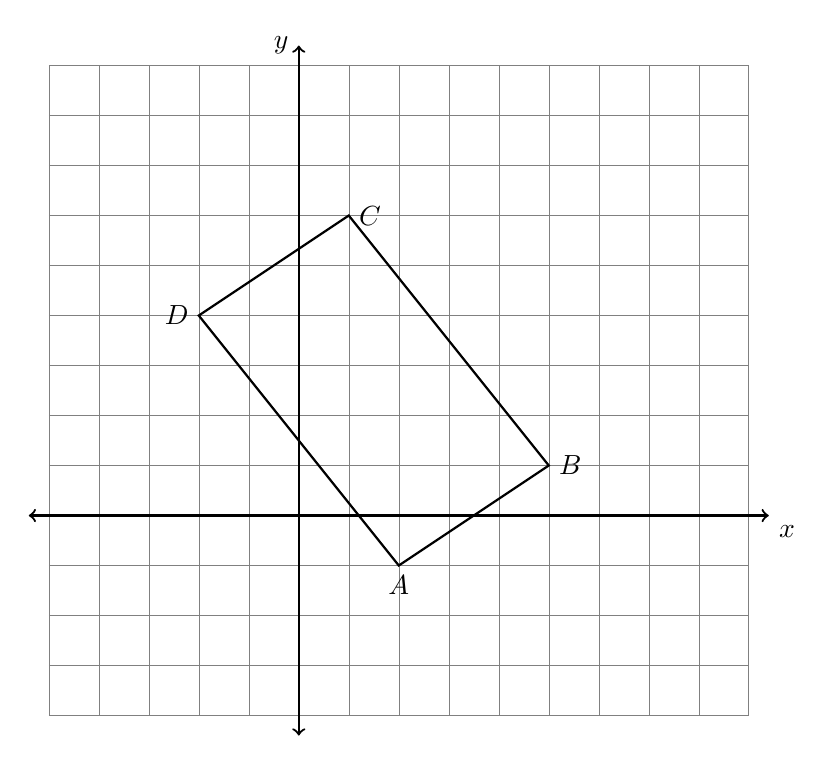
\begin{tikzpicture}[scale=.635]
        \draw [help lines] (-5,-4) grid (9,9);
        \draw [thick, <->] (-5.4,0) -- (9.4,0) node [below right] {$x$};
        \draw [thick, <->] (0,-4.4)--(0,9.4) node [left] {$y$};
        \draw [thick] (2,-1) node[below] {$A$}--
        (5,1) node[right] {$B$}--
        (1,6) node[right] {$C$}--
        (-2,4) node[left] {$D$}--cycle;
      \end{tikzpicture}
    \end{flushright}
  
\newpage
  \subsubsection*{Using the distance formula to prove a parallelogram}
\item In this problem use the following theorem (copy it at the bottom of the page after your calculations): \\*[0.25cm]
    \emph{A quadrilateral is a parallelogram if and only if it's opposite sides are congruent.}\\*[0.5cm]
    Shown below is quadrilateral $ABCD$, $A(2,-1)$, $B(5,1)$, $C(1,6)$, and $D(-2,4)$. \\*[0.25cm]
    Prove it is a parallelogram by
    \begin{enumerate}
      \item finding the length of each of the four sides,
      \item stating which sides are congruent,
      \item copying the theorem as your conclusion.
    \end{enumerate}
    \begin{flushright} %4 quadrant regents grid
      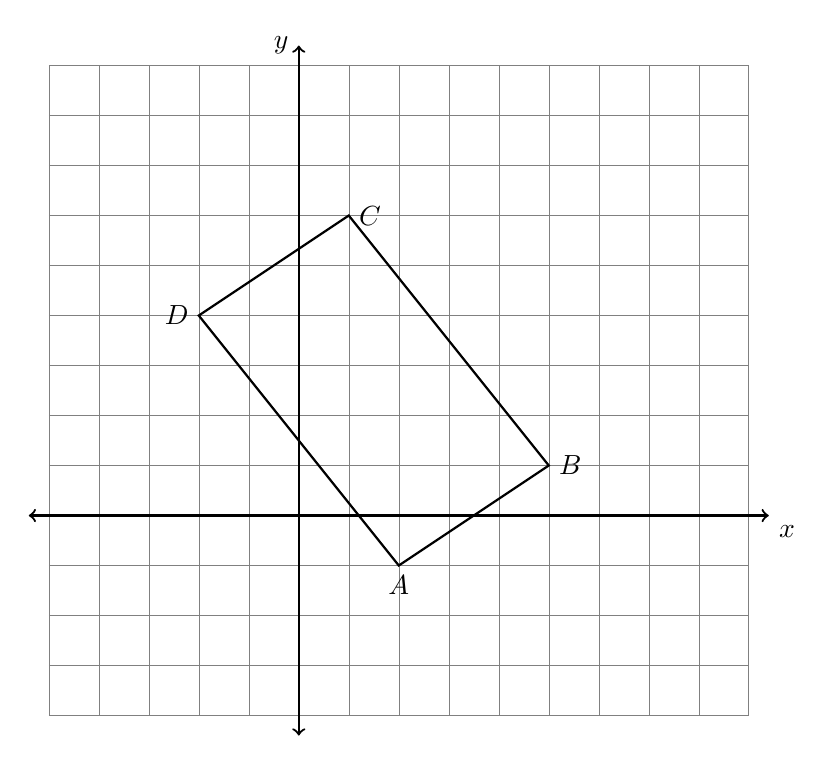
\begin{tikzpicture}[scale=.635]
        \draw [help lines] (-5,-4) grid (9,9);
        \draw [thick, <->] (-5.4,0) -- (9.4,0) node [below right] {$x$};
        \draw [thick, <->] (0,-4.4)--(0,9.4) node [left] {$y$};
        \draw [thick] (2,-1) node[below] {$A$}--
        (5,1) node[right] {$B$}--
        (1,6) node[right] {$C$}--
        (-2,4) node[left] {$D$}--cycle;
      \end{tikzpicture}
    \end{flushright}

    \newpage
\item Given $\overleftrightarrow{AB}$ as shown on the number line, with $A=-3$ and $B=5$. Mark and label the midpoint $M$ between $A$ and $B$?\\[20pt] % Midpoint
      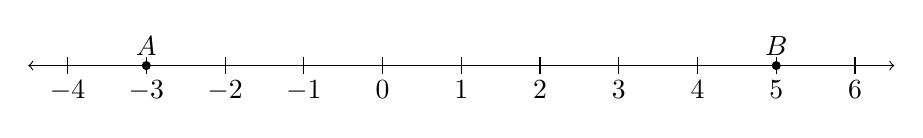
\begin{tikzpicture}
        \draw [<->] (-4.5,0)--(6.5,0);
        \foreach \x in {-4,...,6} %2 leading for diff!=1
          \draw[shift={(\x,0)},color=black] (0pt,-3pt) -- (0pt,3pt) node[below=5pt]  {$\x$};
          \draw [fill] (-3,0) circle [radius=0.05] node[above] {$A$};
          \draw [fill] (5,0) circle [radius=0.05] node[above] {$B$};
      \end{tikzpicture}
      
\item Given two parallel lines and a transversal, as shown below.
    \begin{center}
      \begin{tikzpicture}
        \draw [<->, thick] (1,2)--(9,2);
        \draw [<->, thick] (0,0)--(8,0);
        \draw [<->, thick] (4,-1)--(5.5,3);
        \node at (4.5,0.3) [left]{$5$};
        \node at (4.5,0.3) [right]{$6$};
        \node at (4.3,-0.3) [left]{$7$};
        \node at (4.3,-0.3) [right]{$8$};
        \node at (5.2,2) [above left]{$1$};
        \node at (5.2,2) [above right]{$2$};
        \node at (5,2) [below left]{$3$};
        \node at (5,2) [below right]{$4$};
      \end{tikzpicture}
    \end{center}
    \begin{enumerate}
      \item State the angle corresponding with $\angle 7$. \vspace{0.5cm}
      \item What theorem would justify $m\angle 4 + m\angle 6 =180^\circ$? \rule{5cm}{0.15mm} \vspace{0.5cm}
      \item What theorem would justify $\angle 3 \cong \angle 6$? \rule{7cm}{0.15mm} \vspace{0.5cm}
      \item What theorem would justify $\angle 5 \cong \angle 8$? \rule{7cm}{0.15mm} \vspace{0.5cm}
      %\item Given $m\angle 1 = 117^\circ$ and $m\angle 8 = (4x-3)^\circ$. Find $x$. \vspace{3.5cm}
    \end{enumerate}

\end{enumerate}
\end{document}